% !TEX encoding = UTF-8 Unicode
\documentclass[a4paper]{article}

\usepackage{color}
\usepackage{url}
\usepackage[T2A]{fontenc} % enable Cyrillic fonts
\usepackage[utf8]{inputenc} % make weird characters work
\usepackage{graphicx}
\usepackage{floatrow}
\usepackage{subcaption}
\usepackage[export]{adjustbox}
\usepackage{pgfplots}
\pgfplotsset{compat=1.3}

\pgfplotsset{%
    % #1: index in the group(0,1,2,...)
    % #2: number of plots of that group
    bar group size/.style 2 args={%
        /pgf/bar shift={%
                % total width = n*w + (n-1)*skip
                % -> subtract half for centering
                -0.5*(#2*\pgfplotbarwidth + (#2-1)*\pgfkeysvalueof{/pgfplots/bar group skip})  +
                % the '0.5*w' is for centering
                (.5+#1)*\pgfplotbarwidth + #1*\pgfkeysvalueof{/pgfplots/bar group skip}},%
    },
    bar group skip/.initial=2pt,
    plot 0/.style={blue,fill=blue!30!white,mark=none},%
    plot 1/.style={red,fill=red!30!white,mark=none},%
    plot 2/.style={brown!60!black,fill=brown!30!white,mark=none},%
    plot 3/.style={gray,fill=gray,mark=none},%
}

\usepackage[english,serbian]{babel}
%\usepackage[english,serbianc]{babel} %ukljuciti babel sa ovim opcijama, umesto gornjim, ukoliko se koristi cirilica

\usepackage[unicode]{hyperref}
\hypersetup{colorlinks,citecolor=green,filecolor=green,linkcolor=blue,urlcolor=blue}

\usepackage{listings}

%\newtheorem{primer}{Пример}[section] %ćirilični primer
\newtheorem{primer}{Primer}[section]

\definecolor{mygreen}{rgb}{0,0.6,0}
\definecolor{mygray}{rgb}{0.5,0.5,0.5}
\definecolor{mymauve}{rgb}{0.58,0,0.82}

\lstset{% 
  backgroundcolor=\color{white},   % choose the background color; you must add \usepackage{color} or \usepackage{xcolor}; should come as last argument
  basicstyle=\scriptsize\ttfamily,        % the size of the fonts that are used for the code
  breakatwhitespace=false,         % sets if automatic breaks should only happen at whitespace
  breaklines=true,                 % sets automatic line breaking
  captionpos=b,                    % sets the caption-position to bottom
  commentstyle=\color{mygreen},    % comment style
  deletekeywords={...},            % if you want to delete keywords from the given language
  escapeinside={\%*}{*)},          % if you want to add LaTeX within your code
  extendedchars=true,              % lets you use non-ASCII characters; for 8-bits encodings only, does not work with UTF-8
  firstnumber=1000,                % start line enumeration with line 1000
  frame=single,	                   % adds a frame around the code
  keepspaces=true,                 % keeps spaces in text, useful for keeping indentation of code (possibly needs columns=flexible)
  keywordstyle=\color{blue},       % keyword style
  language=Python,                 % the language of the code
  morekeywords={*,...},            % if you want to add more keywords to the set
  numbers=left,                    % where to put the line-numbers; possible values are (none, left, right)
  numbersep=5pt,                   % how far the line-numbers are from the code
  numberstyle=\tiny\color{mygray}, % the style that is used for the line-numbers
  rulecolor=\color{black},         % if not set, the frame-color may be changed on line-breaks within not-black text (e.g. comments (green here))
  showspaces=false,                % show spaces everywhere adding particular underscores; it overrides 'showstringspaces'
  showstringspaces=false,          % underline spaces within strings only
  showtabs=false,                  % show tabs within strings adding particular underscores
  stepnumber=2,                    % the step between two line-numbers. If it's 1, each line will be numbered
  stringstyle=\color{mymauve},     % string literal style
  tabsize=2,	                   % sets default tabsize to 2 spaces
  title=\lstname                   % show the filename of files included with \lstinputlisting; also try caption instead of title
}

\begin{document}

\title{Projekat GraalVM\\ \small{Seminarski rad u okviru kursa\\Metodologija stručnog i naučnog rada\\ Matematički fakultet}}

\author{Bojan Bardžić, Milica Gnjatović, Pavle Savić, Andrija Urošević\\ 
	\texttt{mi18300@alas.matf.bg.ac.rs}, 
	\texttt{mi18018@alas.matf.bg.ac.rs}, \\ 
	\texttt{mi17169@alas.matf.bg.ac.rs}, 
	\texttt{mi18083@alas.matf.bg.ac.rs}}

%\date{9.~april 2015.}

\maketitle

\abstract{
Danas postoji veliki broj programskih jezika. Neki od njih su veoma aktuelni, neki su zastareli i neefikasni, neki se brzo razvijaju dok se neki više ne održavaju. Ako bismo imali jedan savršen jezik i dalje bi bio problem prevesti sve programe koji su u upotrebi u taj jedan jezik. GraalVM je projekat koji nam pruža mogućnost da izvršavamo aplikacije napisane u više programskih jezika, uključujući i jezike koji se slabo održavaju. Pored toga pokazaćemo kako GraalVM to radi efikasno i zašto ga veliki broj kompanija danas koristi. 
}

\tableofcontents

\newpage

\section{Uvod}
\label{sec:uvod}
GraalVM predstavlja JDK (\emph{Java Development Kit}) visokih performansi\cite{graalvmintroduction}. GraalVM omogućava ubrzanje izvršavanja uz korišćenje manje resursa. Java aplikacije je ovim moguće prevesi na dva načina: AOT(\emph{Ahead Of Time}) i JIT ( \emph{Just In Time}). Pored Jave, neki od jezika koje GraalVM podržava su(slika~\ref{fig:jezici}): 
\begin{itemize}
	\item JavaScript i Node.js
	\item Python
	\item Ruby
	\item R
	\item LLVM jezici poput C-a i C++-a
	\item WebAssembly\\
\end{itemize}

U ovom radu prolazimo kroz osnovne elemente i ciljeve ovog projekta, šta je to inovativno uvedeno i gde se sve koristi. 

\begin{figure}
	\caption{Podržani jezici.}
	\begin{subfigure}{\linewidth}
		
\includegraphics[width=0.16\linewidth]{imgs/java_logo.png}
		
\includegraphics[width=0.16\linewidth]{imgs/c_logo.png}
		
\includegraphics[width=0.16\linewidth]{imgs/cpp_logo.png}
		
\includegraphics[width=0.16\linewidth]{imgs/r_logo.png}
		
\includegraphics[width=0.16\linewidth]{imgs/python_logo.png}
		
\includegraphics[width=0.16\linewidth]{imgs/ruby_logo.png}
	\end{subfigure}
	
	\begin{center}
		
\includegraphics[width=0.5\linewidth]{imgs/graalvm_logo.png}	
	\end{center} 
	
	\begin{subfigure}{\linewidth}
		
\includegraphics[width=0.16\linewidth]{imgs/js_logo.png}
		
\includegraphics[width=0.16\linewidth]{imgs/nodejs_logo.png}
		
\includegraphics[width=0.16\linewidth]{imgs/clojure_logo.png}
		
\includegraphics[width=0.16\linewidth]{imgs/kotlin_logo.png}
		
\includegraphics[width=0.16\linewidth]{imgs/scala_logo.png}
		
\includegraphics[width=0.16\linewidth]{imgs/wa_logo.png}
	\end{subfigure}
	\label{fig:jezici}
\end{figure}
Upotrebom ovog alata je omogućeno efikasnije korišćenje više jezika na jednom projektu. U projektu je moguće kodom pisanim u jednom jeziku pozivati funkcije pisane u drugom jeziku. Dopušteno je deljenje struktura podataka između kodova pisanih u različitim jezicima. Zbog toga sakupljač otpadaka radi na celom projektu, bez obzira na to koliko različitih jezika je korišćeno. Ovim je omogućeno i jednostavnije debagovanje.

Ovaj alat je koristan u radu sa mikroservisnom arhitekturom. Nekolicina okvira za rad sa Java mikroservisima je već prihvatila ovu platformu. Između ostalih to su Micronaut, Spring, Helidon i Quarkus \cite{graalvm}. 

Još jedna od mogućnosti koje GraalVM nudi je implementiranje novih jezika i alata korišćenjem biblioteke Truffle \cite{graalvmtruffle}.

GraalVM je implementiran u Javi. Čine ga Java Virtuelna Mašina --- JVM i Java Development Kit --- JDK.\ Ovaj alat omogućava brže izvršavanje koda, a da se pri tome koristi manje memorije.

GraalVM je dostupan na Linux, Windows i MacOS operativnim sistemima \cite{graalvmintroduction}.

Dostupna su dva izdanja GraalVM-a:

\begin{description}
	\item [Community edition] je otvorenog koda i dostupno je na github-u. Korisnici mogu doprineti razvoju ove verzije \cite{graalvmCommunity}.
	\item [Enterprise edition] razvija i licencira kompanija Oracle \cite{graalvmEnterprise}.
\end{description}

GraalVM je podržan od strane razvojnih okruženja i protokola za debagovanje. Neka od tih okruženja su Eclipse, NetBeans, IntelliJ IDEA i Visual Studio Code. Ova okruženja su posebno dobra jer podržavaju sve jezike koje podržava i GraalVM.\ Ovaj alat obezbeđuje ugrađen Crome DevTools Protocol, Debug Adapter Protocol (DAP) i Language Server Protocol (LSP), čime je omogućeno debagovanje JavaScript, R i Ruby kodova.

\subsection{Istorijski razvoj}
\label{subsec:istorija}

Projekat GraalVM je istraživački projekat koji razvija Oracle labs. Od 2012. preko šezdeset naučnih radova je izdato od strane razvojnog tima. Jedan od prvih radova koji iznosi ideju ovog projekta je \textit{One VM to rule them all} \cite{onevmtorulethemall}.

Java Virtuelne mašine poput Oracle Java HotSpotVM i IBM Java VM postoje više od dve decenije. Međutim nije postojala virtuelna mašina koja bi omogućila efikasno izvršavanje kodova pisanih u različitim jezicima. Cilj ovog projekta je bio da se napravi objedinjena virtuelna mašina koja bi ovo omogućila.

Prva verzija GraalVM 19.0 je objavljena u maju 2019. Trenutno najnovija verzija je GraalVM 22.3.0, objavljena u oktobru 2022. \cite{graalvmreleases}.

\section{Šta obuhvata projekat?}
\label{sec:projekat}

Kao što je prethodno navedeno, ovaj projekat uvodi neke nove koncepte. Sam projekat obuhvata više komponenti koje ga čine korisnim i inovativnim. U ovom odeljku se govori o tome kako GraalVM zamenjuje JVM, i mogućnostima koje nudi Truffle.

\subsection{GraalVM kao zamena za JVM}
\label{sub:GraalVMJVM}

Jedna od prednosti GraalVM je što se može koristiti umesto Java virtuelne mašine, on može da pokreće Java, Scala i Kotlin programe, kao i sve ostale programe pisane u jezicima koje se prevode u Java bajt kod. Od 2019. može se izvršavati na Linux-u, a od verzije 20.1.0 ima podršku i za Windows.

Još jedna od prednosti koja se pripisuje GraalVM-u su odlične performanse. Neke demonstracije pokazuju da se Ruby program izvršava i do 30 puta brže od originalne implementacije \cite{graalvmbenchmark}. Detaljnija testiranja su ipak pokazala da se u proseku Ruby kod izvšava oko 30\% brže na GraalVM, što je i dalje obećavajući rezultat \cite{whataboutgraalvm}.

Kada su testirani Java programi rezultati su bili manje optimistični, performanse GraalVM-a su okvirno slične Oracle-ovom HotSpot kompajleru \cite{graalvm}. Ovo samo po sebi ne predstavlja loš rezultat, ali ne predstavlja ni neki revolucionarni napredak u odnosu na sadašnje tehnologije. U svakom slučaju, GraalVM će biti brži od klasične JVM.\ Iako ne predstavlja poboljšanje u odnosu na HotSpot VM, prednost GraalVM-a je u tome što je nov kompajler nad kojim nije vršena optimizacija preko dvadeset godina, kao što je to slučaj sa HotSpot-om. Još jedna prednost u odnosu na prethodne kompajlere je to što je pisan u Javi za razliku od prethodnih kompajlera koji su pisani u jezicima C i C++. To omogućava lakše proširenje i optimizaciju od strane Java programera.

\subsection{Truffle --- kompajler za kompajlere}
\label{sub:truffle}

Truffle je biblioteka otvorenog koda za pravljenje alata i implementacija programskih jezika kao interpretera za samomodifikujuća apstraktna sintaksna stabla \cite{graalvm}. On nam dozvoljava da pravimo interpretere bez većih problema. Osnovna prednost njegovog korišćenja je u tome što se interpretirani kod izvršava podjednako brzo kao i program dobijen prevođenjem. Truffle je korišćen za pisanje interpretera za jezik JavaScrpit u GraalVM-u. Pri izvršavanju koda potrebno mu je neko vreme da se ``zagreje'', ali kada dostigne optimalne performanse one su okvirno iste kao kod kompajlera V8 kompanije Google.

Optimizacija koda je zasnovana na ideji parcijalne evaluacije \cite{graalvm}. Truffle uzima interpreter koji smo mu dali i naš program, zatim koristi JIT kompajler i promenom sintaksnog stabla vrši optimizaciju koda. Da bi se utvrdilo koje optimizacije je potrebno izvršiti program mora prvo biti pokrenut, zbog toga se javlja sporije vreme izvršavanja na početku.

Takođe, pri pisanju interpretera koristeći Truffle možemo da naglasimo gde i kada želimo da kod bude optimizovan. U nekim slučajevima promena u izvornom kodu može da dovede do greške u programu i u tom slučaju je potrebno deoptimizovati kod. Sve ove optimizacije i izbacivanja nekorišćenog koda iz našeg programa dovode do velike brzine izvršavanja.

Standardni podržani jezici za Truffle su JavaScript zajedno sa okruženjem Node.js, kao i Ruby, R i Python. Pored toga, Truffle ima u sebe ugrađen Sulong koji može da izvršava LLVM bitkod i tako izvšava programe pisane na jezicima kao što su C, C++, C\#, D, Lua i FORTRAN.\ Ovim se omogućava da GraalVM izvšrava veliki broj različitih programskih jezika, kao i da se funkcije iz jednog jezika pozivaju u drugom jeziku, omogućavajući time veću fleksibilnost pri pisanju programa.

\subsection{Izvršavanje mašinskog koda na cloud-u}
\label{sub:cloud}

Jedna od glavnih funkcionalnosti koje uvodi ovaj projekat jeste kompajliranje Java programa sa bajt koda na mašinski kod. Ovo je funkcionalnost koja nam dozvoljava tako nešto prvi put od kako postoji programski jezik Java. Jedan od slučajeva upotrebe je izvšavanje mikroservisa na cloud-u \cite{sipek21}.

Mikroservisi se sada kompajliraju u izvršni fajl i time je eliminisana potreba da na serverskoj strani mora postojati Java virtuelna mašina. Ovo dovodi do smanjenja zauzeća memorije na serveru. Još jedna prednost ovog pristupa je u tome što više nije potrebno da se za naše programe učitava mnoštvo Java klasa pri pokretanju, od kojih većina neće biti upotrebljena. Ovo dovodi do bržeg izvršavanja naših programa na serverskoj strani i sprečava sporo izvšavanje pri prvom pokretanju. 

\begin{figure}
	\begin{center}
	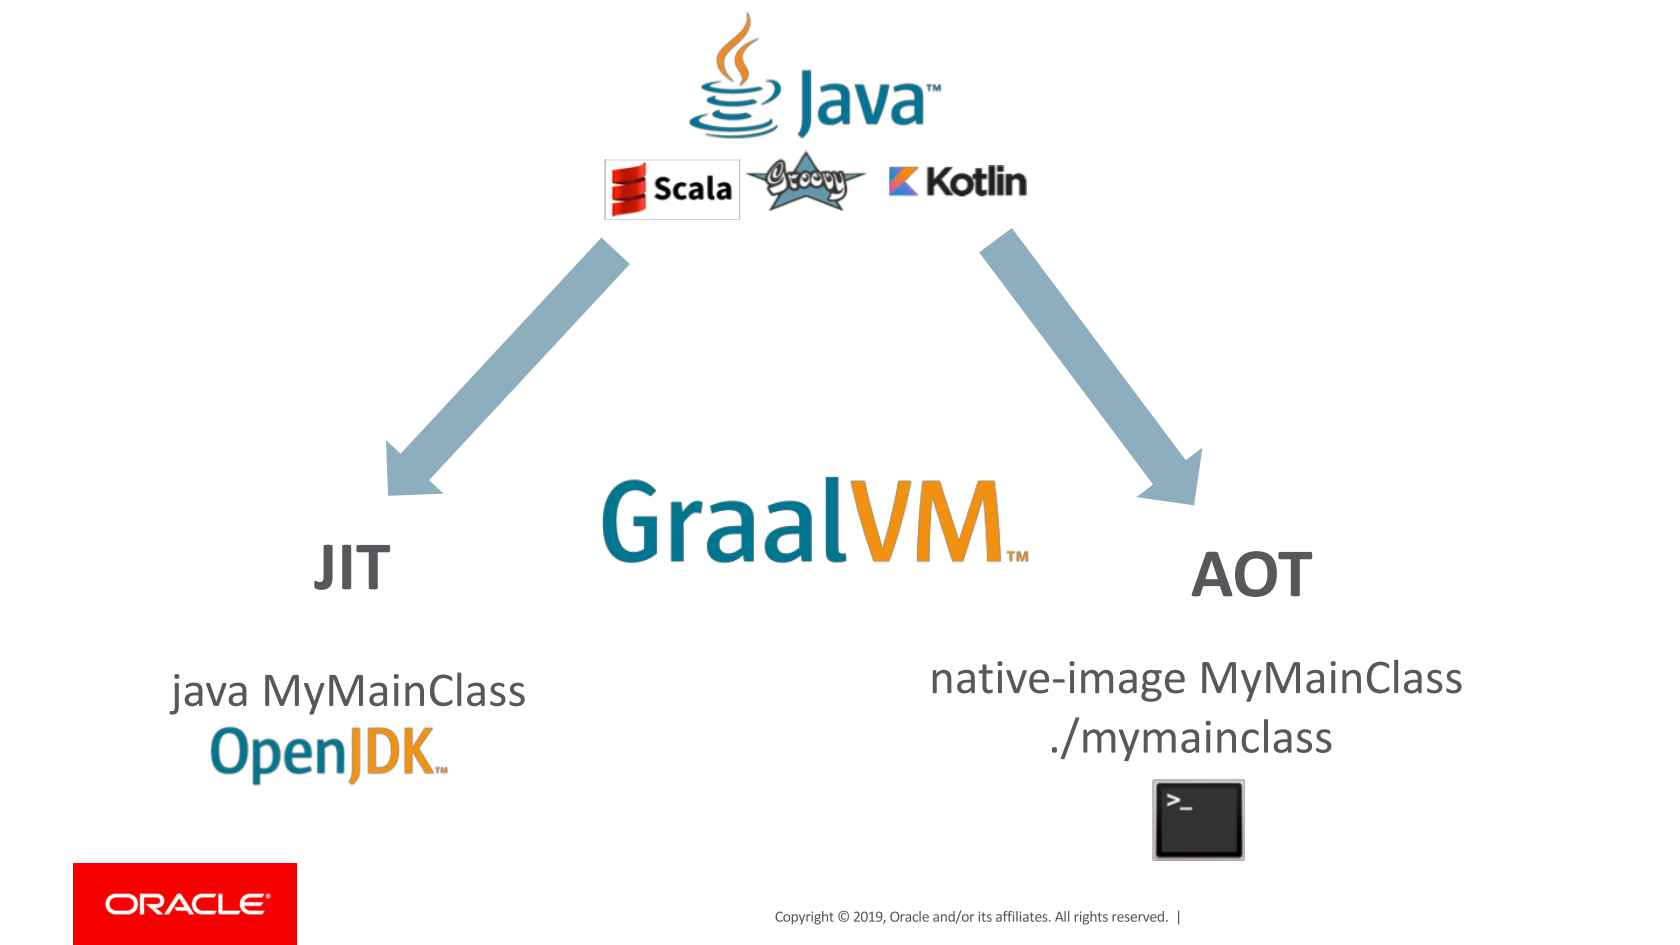
\includegraphics[scale=0.25]{imgs/run_java.jpg}
	\end{center}
	\caption{Dva načina za prevođenje Java programa korišćenjem GraalVM-a.}
	\label{fig:runjava}
\end{figure}


\subsection{Espresso --- Java on Truffle}
\label{sub:espresso}

Postoje dva ustaljena načina za prevođenje koda napisanog u Java-i korišćenjem GraalVM-a kompajlera, to su JIT (Just-In-Time) i AOT (Ahead-of-Time) (slika~\ref{fig:runjava}).\ Od verzije 21.0 uvedena je nova komponenta, nazvana \emph{espresso}. \emph{Espresso} predstavlja implementaciju JVM specifikacije, koja je napisana u Java-i pomoću Truffle radnog okvira. Ova komponenta nije podrazumevano deo GraalVM-a ali može se lako instalirati korišćenjem \emph{GraalVM Updater tool}-a \cite{graalvm}. Na raspolaganju je i za GraalVM distribucije zasnovane na Java-i 8, kao i na Java-i 11 tako da se može koristiti kao zamena za JVM po izboru.

\emph{Java on Truffle} režim izvršavanja pokreće Java kod preko bajtkod interpretera implementiranog korišćenjem Truffle-a (slika~\ref{fig:javaontruffle}). Na ovaj način Java (i drugi JVM zasnovani jezici) pokreću se na isti način kao tradicionalni interpretirani i LLVM jezici koje GraalVM podržava. Ovo omogućava potpunu interoperabilnost sa njima --- poliglot programiranje \footnote{Poliglot programiranje je praksa pisanja koda u više jezika da bi se iskoristile dodatne mogućnosti svakog jezika. Više reči o tome će biti u delu \ref{sub:poliglot}.} \cite{grooteman2017java, graalvm}. Iz tog razloga se mogu pozivati funkcije napisane u ovim jezicima u Java-i, kao i Java funkcije u drugim Truffle jezicima. Pri ovakvom izvršavanju podaci se nalaze u zajedničkom memorijskom prostoru.

Činjenica da je \emph{Java on Truffle} implementiran u Java-i (eng. \emph{self-hosting}) smatra se ``Svetim gralom'' u razvoju JVM-a. Da bi \emph{Java on Truffle} mogla da pokrene Java kod neophodan joj je pristup JCL-u (Java Class Library), nativnim bibliotekama i metodama koje pruža JDK (Java Development Kit). \emph{Java on Truffle} ponovno koristi Java Archive datoteke i nativne biblioteke iz GraalVM distribucije \cite{grooteman2017java}. Kao posledica \emph{self-hosting}-a \emph{Java on Truffle} jeste metacirkularna VM\footnote{Metacirkularna VM može pokretati samu sebe nekoliko nivoa u dubinu, pri čemu svakim silaskom postaje nešto sporija.}. Druga prednost ovoga je da je izvorni kod razumljiv Java programerima. Ovaj nivo transparentnosti, kroz zajednicu otvorenog koda, čini \emph{Java on Truffle} projektom koji se ubrzano razvija i unapređuje.

\emph{Java on Truffle} istovremeno je JVM i Java program, što znači da može biti pokrenuta unutar drugog Java programa. Ovo daje mogućnost razdvajanja aplikacije u komponente sa zajedničkom funkcionalnošću kako bi se proces programiranja učinio lakšim za upravljanje i podigla ponovna upotrebljivost koda. Na ovaj način može se ugraditi Java 8 kontekst u Java 11 aplikaciju i obrnuto, koristeći \emph{GraalVM Polyglot API} \cite{graalvm}. Na primer ako su na raspolaganju obe distribucije (JDK 11 i JDK 8),
\emph{Java on Truffle} može biti pokrenuta kao Java 8 aplikacija, a potom može biti iskorišćena za pokretanje Java 11 bajtkoda i obrnuto \cite{grooteman2017java}. Ako postoji biblioteka dostupna samo za Java-u 8, sada je moguće prebaciti se na noviji JDK i, uz manje programerske napore da se uspostavi interoperabilnost, koristiti je u Java 11 aplikaciji. Takođe ovime se povećava nivo izolovanosti \emph{host} VM-a i Java programa koji se pokreće. Ovo povećava bezbednost pri izvršavanju manje pouzdanog ili nepoznatog koda \cite{graalvm}.

\emph{Java on Truffle} ima sve osnovne komponente JVM, pa tako i JDWP (Java Debug Wire Protocol) koji služi za komunikaciju između debagera i ciljnog JVM-a. Nije potrebno ništa dodatno konfigurisati da bi se debagovale aplikacije pokrenute preko \emph{Java on Truffle}. Moguće je korišćenje debagera integrisanog razvojnog okruženja \cite{graalvm}. Još jedna pogodnost koju nam \emph{Java on Truffle} nudi jesu unapređene mogućnosti za redefinisanje klasa u fazi izvršavanja (eng. \emph{Hot Swap}) u odnosu na HotSpot JVM tokom debagovanja. Neke od podržanih promena u verziji GraalVM 21.0:
\begin{itemize}
    \item dodavanje i brisanje metoda i konstruktora klasa;
    \item dodavanje i brisanje metoda iz interfejsa;
    \item promena prava pristupa za metode i konstruktore;
    \item promena lambda izraza;
    \item dodavanje i brisanje anonimnih klasa.
\end{itemize}
Novije verzije donele su i mogućnost manipulacije poljima i hijerarhijama klasa. Nešto što treba očekivati u narednim verzijama jeste mogućnost promene enumeratorskih klasa \cite{graalvm}.

\emph{Java on Truffle} i dalje je eksperimentalna tehnologija. Maksimalne performanse su trenutno 2-3 puta sporije nego kod HotSpot-a. Vreme pokretanja je takođe nedovoljno optimizovano i još uvek nije na nivou brzine koju nudi standardno GraalVM JIT prevođenje \cite{graalvm}. Treba imati na umu da ovo nisu reprezentabilni podaci za ono što se očekuje od \emph{Java on Truffle} u bliskoj budućnosti. Poboljšanje performansi jeste nešto na šta je razvojni tim trenutno najviše fokusiran. Pored toga radi se na podršci za Java agente, kao i na implementaciji boljih protokola interakcije sa drugim jezicima u okviru poliglotskih aplikacija \cite{graalvm}.


\begin{figure}
	\begin{center}
	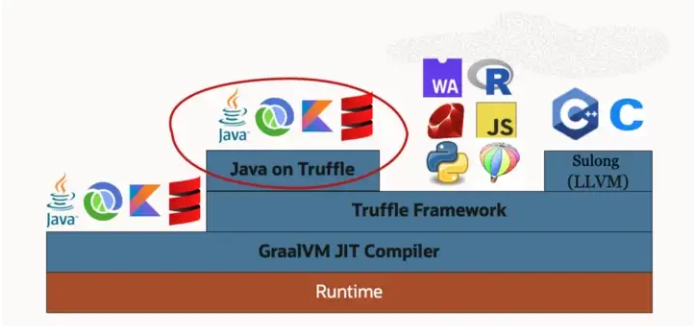
\includegraphics[scale=0.35]{imgs/java_on_truffle.png}
	\end{center}
	\caption{\emph{Java on Truffle} u GraalVM ekosistemu.}
	\label{fig:javaontruffle}
\end{figure}

\section{Karakteristike}
\label{sec:karakteristike}

Projekat \emph{GraalVM} karakterišu visoke performanse, poliglot programiranje, \emph{GraalVM AOT} (\emph{ahead-of-time}) kompilacija u \emph{Native Image}, napredni alati \cite{graalvm}. U narednim podsekcijama će biti opisani svaki od ovih karakteristika.

\subsection{Visoke performanse}
\label{sub:perf}

Jedna od karakteristika kojom \emph{GraalVM} može da se pohvali, jesu veoma visoke performanse u odnosu na \emph{OracleJDK}, i \emph{OpenJDK}. 

Šipek i drugi \cite{vsipek19} pokretanjem \emph{DaCapo} benčmarka \cite{dacapo} pokazuju da \emph{GraalVM CE}, i posebno \emph{GraalVM EE} daju bolje performanse u odnosu na \emph{JDK10} i \emph{JDK11} (slika~\ref{fig:dacapo}). Na testu h2 \emph{GraalVM CE} daje rezultate i za 19.8\% bolje od \emph{JDK11}. Na drugim testovima vidimo malo poboljšanje \emph{GraalVM} kompajlera u odnosu na \emph{JDK}, ali i to da \emph{JDK} u malom broju testova daje bolje rezultate. Pored toga, uočavamo da \emph{GraalVM EE} u odnosu na \emph{GraalVM CE} nad h2 testovima daje rezultate bolje i za 47.06\%, što je veoma velika razlika. Što se stabilnosti tiče, tj.\ veličine standardne devijacije u performansama, najbolje se pokazuje \emph{JDK11}, a najgore \emph{GraalVM EE}.

\begin{figure}
\begin{center}
    \begin{tikzpicture}
    \begin{axis}[
        width=0.85\textwidth,
        x tick label style={/pgf/number format/1000 sep=},
        ylabel=Prosečno vreme u milisekundama $(ms)$,
        enlargelimits=0.15,
        legend style={at={(0.5,-0.15)},
        anchor=north,legend columns=-1},
        ybar,
        bar width=7pt,
        xtick={0,1,2,3,4,5},
        xticklabels={h2, lusearch, xalan, pmd, sunflow, jython},
        ]
        \addplot[plot 0,bar group size={0}{4}]
        coordinates {(0,4494.95) (1,2683.40) (2,863.32) (3,138.23) (4,5062.05) (5,6652.86)};
        \addplot[plot 1,bar group size={1}{4}]
        coordinates {(0,5327.10) (1,2757.10) (2,277.41) (3,194.61) (4,5626.25) (5,7038.34)};
        \addplot[plot 2,bar group size={2}{4}]
        coordinates {(0,10821.85) (1,2874.50) (2,870.72) (3,201.95) (4,5417.25) (5,6433.60)};
        \addplot[plot 3,bar group size={3}{4}]
        coordinates {(0,9550.05) (1,2886.15) (2,232.51) (3,276.76) (4,6151.25) (5,6672.10)};
        \legend{GraalVM EE, GraalVM CE, JDK10, JDK11}
    \end{axis}
\end{tikzpicture}
\end{center}
    \caption{\emph{DaCapo} benčmark na \emph{GraalVM EE, GraalVM CE, JDK10, JDK11}.}
\label{fig:dacapo}
\end{figure}

Pored \emph{DaCapo} benčmarka razvija se i novi \emph{Renaissance} benčmark. \emph{Renaissance} benčmark obećava prednosti nad konkurencijom, tako što koristi moderna, realna, konkurentna, i objektno orijentisana preopterećenja kako bi prikazao bolju sliku performansi kompajlera \cite{prokopec19}. Pokretanjem ovih testova uočeno je značajno poboljšanje \emph{GraalVM JIT} kompajlera u odnosu na \emph{JDK11} i \emph{JDK17} \cite{renaissance}.

Poboljšanje u performansama je vidljivo i na drugim benčmarkovima. Tako je uočeno da \emph{Scala} ima bolje performanse kada se koristi \emph{GraalVM} optimizator, takođe i na \emph{DaCapo} benčmarkovima \cite{stadler13, dacapo}. \emph{Cloud} servisi, takođe, dobijaju značajno unapređenje \cite{sipek21}. 

Treba napomenuti da postoje istraživanja koja pokazuju da \emph{GraalVM} ne pokazuje značajna poboljšanja u odnosu na \emph{JDK}. Fong i drugi \cite{fong21} pokazuju da u nekim slučajevima \emph{GraalVM} daje podjednake čak i lošije rezultate. 

\subsection{Native Image}
\label{sub:nim}

\emph{GraalVM} pruža tehnologiju \emph{Native Image} \cite{graalvm}. \emph{Native Image} predstavlja izvršivi binarni fajl koji je dobijen \emph{GraalVM AOT} kompilacijom. Ovaj fajl sadrži klase aplikacije, klase biblioteka, zavisne klase i statički linkovan kod iz \emph{JDK}-a. Dobijeni izvršivi fajl se ne pokreće na \emph{Java VM}, već on uključuje potrebne dodatke iz \emph{Java VM}-e. Za rezultat imamo da se dobijeni program pokreće brže jer učitava samo potrebne klase. Program je sigurniji, jer se sa manjom bazom koda mogućnost nastanka greške smanjuje. Program se lako isporučuje, jer se kapacitet kontejnera smanjuje.

\subsection{Poliglot programiranje}
\label{sub:poliglot}

Jedna od ključnih karakteristika koju \emph{GraalVM} pruža jeste poliglot programiranje \cite{graalvm}. Poliglot programiranje podrazumeva da programeri za rešavanje nekog problema koriste odgovarajući programski jezik. Tako rešene probleme onda koriste u projektu. Mehanizmi integracije više programskih jezika stvara dodatne kompleksnosti. Postoje mnogi radovi koji tvrde da se efikasnost programera, samim tim i programa smanjuje uvođenjem više jezičke strukture \cite{peterson21, hao20}. Sa ciljem rešavanja ovog problema \emph{GraalVM} pruža \emph{TruffleVM} koji obećava lako i jednostavno prenošenje podataka, i korišćenje konstrukcija nekog programskog jezika unutar nekog drugog programskog jezika \cite{grimmer15}.

\subsection{Napredni alati}
\label{sub:alati}

U tabeli~\ref{alati} su prikazani dostupni alati i njihove funkcionalnosti unutar projekta \emph{GraalVM} \cite{graalvm}.

\begin{table}
    \centering
    \begin{tabular}{|l|l|}
        \hline
        VS Code Extensions & Radno okruženje unutar VS Code-a\\
        \hline
        GraalVM Dashboard & Vizuelna reprezentacija delova projekta\\
        \hline
        Chrome Debugger & Debager za JS, Ruby, R i Python\\
        \hline
        VisualVM & Profajler, monitor, aktivne niti\ldots\\
        \hline
        GraalVM Insight & Praćenje programa u izvršavanju\\
        \hline
        Ideal Graph Visualizer & Graf faza kompilacija\\
        \hline
    \end{tabular}
    \caption{Napredni alati unutar Projekta \emph{GraalVM}.}
    \label{alati}
\end{table}

\section{Kompanije koje koriste GraalVM}
\label{sec:comp}

\begin{description}
	\item[Facebook] \hfill \\
	Društvena mreža Facebook ima ogroman broj korisnika zbog čega je jako bitno da se kod dobro skalira i brzo izvršava.
	Na serverskoj strani koristi Javu i Spark okvir za rad sa velikom količinom podataka. Prelazak sa Oracle JDK-a i Open JDK-a na GraalVM se sveo samo na promenu runtime okruženja, bez ikakvih promena u kodu. Izmereno je prosečno ubrzanje 1.1 puta korišćenjem Community verzije i ubrzanje 1.42 puta korišćenjem Enterprise verzije GraalVM-a. \cite{graalvmusecases}
	
	\item[Twitter] \hfill \\
	Kao i Facebook, Twitter je društvena mreža sa milionima korisnika. Sa porastom broja korisnika bile su neophodne promene koje bi omogućile brzo izvršavanje uz minimalne troškove. Većina mikroservisa Twitter-a je implementirano u jeziku Scala. Prelaskom na GraalVM je omogućeno 8-11\% ušteda na procesoru. \cite{graalvmusecases}	
	
	\item[Standard Chartered Bank] \hfill \\
	Ova kompanija je između ostalog koristila Javu, Python sa SpringBoot okvirom kako bi obezbedila stabilnost i robusnost programa. Pre par godina kompanija je odlučila da svoju aplikaciju prebaci u cloud, što je donelo nove izazove. GraalVM je obezbedio jednostavan prelazak na cloud time što podržava tehnologije koje su programi već koristili. GraalVM je omogućio skalabilnost i ubrzanje od 7\% \cite{graalvmusecases}.
		
	\item[Goldman Sachs]  \hfill \\
        Goldman Sachs je investiciona banka. Ova kompanija ima svoj programski jezik Slang koji ima funkcije pogodne za njihove potrebe. Jezik je dosta glomazan i potrebno mu je unapređenje. Prevođenje celog koda u neki drugi jezik bi bilo previše zahtevno. GraalVM i Truffle su omogućili unapređenje i ubrzanje izvršavanja koda pisanog u Slang-u, a da je pri tom napisana minimalna količina novog koda \cite{graalvmusecases}.
	
	\item[Nvidia]  \hfill \\
	Nvidia je jedan od najvećih proizvođača grafičkih kartica. Iako neki jezici jednostavno mogu da ubrzaju izvršavanje korišćenjem grafičke kartice, za neke druge to može biti izazovno. GraalVM i Truffle su omogućili kreiranje grCuda jezika koji je kao dodatni jezik GraalVM-a.\ Kako jezici u GraalVM-u efikasno komuniciraju međusobno tako je omogućena jednostavna komunikacija sa jezikom grafičke kartice i grafičkom karticom \cite{graalvmusecases}.
	
	\item[Politie]  \hfill \\
	Holandska policija je imala monolitnu aplikaciju koja je koristila između ostalog TypeScript, Angular, Scala, Axon, SpringBoot, Slick i R. Ova aplikacija je obrađivala velike količine podataka u realnom vremenu, ali to je bilo veoma sporo. Cilj je bio preći na cloud i mikroservisnu ahitekturu, a pri tom ne implementirati sve ispočetka. GraalVM je omogućio ovaj prelazak i ubrzanje, pri čemu je ostao značajan deo starog koda \cite{graalvmusecases}.
\end{description}

\section{Zaključak}
\label{sec:zakljucak}


Projekat GraalVM donosi sa sobom mnogo novina, između ostalog imamo efikasan JDK pisan za Javu i ostale jezike zasnovane na JVM-u. Pored toga ima i podršku za poliglot programiranje, kao i efikasno interpretiranje. 

Truffle nam nudi mogućnost pravljenja interpretera za potpuno nove jezike, kao i za stare koji su postali neefikasni i skupi za održavanje.

GraalVM se pokazao kao dobra alternativa JVM. Kroz benčmarkove smo utvrdili da GraalVM daje dobre performanse. 

Ovaj projekat je pokazao veliki potencijal u pogledu optimizacije i dopunjavanja kompajlera.

O kvalitetu ovog projekta nam govori činjenica da ovaj alat koriste mnoge velike kompanije, između ostalih, Oracle, Facebook, Twitter, i Nvidia. Posebno je dobro što imamo veliku kompaniju koja stoji iza projekta kao i zajednicu koja ga održava.

GraalVM je u ovom radu predstavljen kao nešto izuzetno korisno i efikasno. Dalje se postavlja pitanje `Da li GraalVM ima konkurenciju?'.

Trenutno nema projekata sličnih ovome. Prema tome, glavna konkurencija ostaju kompajleri i alati za pojedinačne jezike. Danas se kao glavna konkurencija navode Amazon Coretto, Red Hat, OpenJDK, Azul Platform Prime i Microsoft Build of OpenJDK. 

\addcontentsline{toc}{section}{Literatura}
\appendix
\bibliography{seminarski} 
\bibliographystyle{plain}

\end{document}
